\documentclass[11pt,a4paper]{article}
\usepackage[margin=20mm]{geometry}
\usepackage[T1]{fontenc}
\usepackage[utf8]{inputenc}
\usepackage{array,booktabs,longtable,tabularx}
\usepackage{enumitem}
\usepackage{xcolor}
\usepackage{hyperref}
\usepackage{tikz}
\usepackage{pgfplots}
\pgfplotsset{compat=1.18}

\definecolor{navy}{HTML}{17365D}
\definecolor{blue}{HTML}{4472C4}
\definecolor{green}{HTML}{70AD47}
\definecolor{amber}{HTML}{ED7D31}
\definecolor{red}{HTML}{C00000}
\definecolor{lightgray}{HTML}{E7E6E6}
\hypersetup{colorlinks=true,linkcolor=navy,urlcolor=blue}
\setlist{nosep,leftmargin=*}
\setlength{\parindent}{0pt}
\setlength{\parskip}{5pt}
\setlength{\emergencystretch}{2em}
\renewcommand{\arraystretch}{1.15}

\newcommand{\status}[2]{\textcolor{#1}{\textbf{#2}}}
\newcommand{\repo}{\texttt{Trishul}}

\title{\textbf{Trishul GRC/TPRM Platform}\\Implementation Status and Delivery Outlook}
\author{Repository assessment against the GRC/TPRM Platform Concept Note v1.0}
\date{Assessment date: 7 August 2026}

\begin{document}
\maketitle

\begin{center}
\fcolorbox{navy}{lightgray}{\parbox{0.91\textwidth}{
\textbf{Headline assessment.} The repository contains a credible secure SaaS and
Deployment Assurance foundation, but it is not yet the complete GRC/TPRM product
described by the concept note. Estimated completion is \textbf{29\% of the whole
concept-note scope}, \textbf{45\% of the stated MVP differentiators}, and
\textbf{65\% of the platform/security foundation}. These are evidence-weighted
engineering estimates, not test coverage or contractual completion figures.
}}
\end{center}

\tableofcontents
\newpage

\section{Executive summary}

The strongest implemented areas are multi-tenant foundations, engagement-scoped
auditor access, deterministic Deployment Assurance, risk/task linkage, immutable
audit records, and infrastructure hardening. The codebase has 139 collected Python
tests, a small React client, Kubernetes/OpenShift/AWS deployment profiles, and
Terraform for private EKS, workload identity, immutable audit checkpoints, and
pilot-light disaster recovery.

The largest gaps are the general-purpose evidence intelligence pipeline, full
framework content, policy lifecycle, third-party risk management, executive and
auditor portals, scoring/history, workflow/report scheduling, production
integrations, and AI evaluation data. The existing frontend is a functional pilot
screen rather than the persona-specific product described in the concept note.

With the concept note's assumed cross-functional team of 10--14 people, a sensible
forecast is:

\begin{itemize}
  \item pilot hardening and live AWS proof by \textbf{September 2026};
  \item a defensible MVP cut line by \textbf{January--February 2027};
  \item expanded GRC/TPRM capability by \textbf{May--June 2027}; and
  \item the wider concept-note scope by \textbf{September--October 2027}.
\end{itemize}

The final date has roughly \textbf{$\pm$25\% uncertainty}. A team of 4--6 would
more realistically require 18--24 months. These requirements are a product roadmap,
not a single defect that can be ``fixed'' on one date.

\section{Assessment method}

The assessment maps the 53-page concept note to repository models, APIs, tests,
frontend behavior, deployment manifests, Terraform, and operational runbooks.
Scores represent the approximate fraction of required behavior for which concrete
repository evidence exists, adjusted down where the implementation is only a data
model, generic CRUD API, pilot UI, or unproven infrastructure definition.

\begin{center}
\begin{tabular}{cl}
\toprule
Score & Interpretation \\
\midrule
90--100\% & Implemented and substantially verified \\
50--89\% & Substantial implementation; important gaps remain \\
20--49\% & Partial foundation or narrow pilot path \\
1--19\% & Nascent implementation \\
0\% & No material repository evidence found \\
\bottomrule
\end{tabular}
\end{center}

The 29\% headline is the simple mean of sixteen product and cross-cutting
workstreams. It deliberately avoids converting test counts or lines of code into
product completion. Production acceptance still requires traceability to a formal
SRS, stakeholder sign-off, content validation, security testing, load testing, and
live operational exercises.

\section{Progress by workstream}

\begin{center}
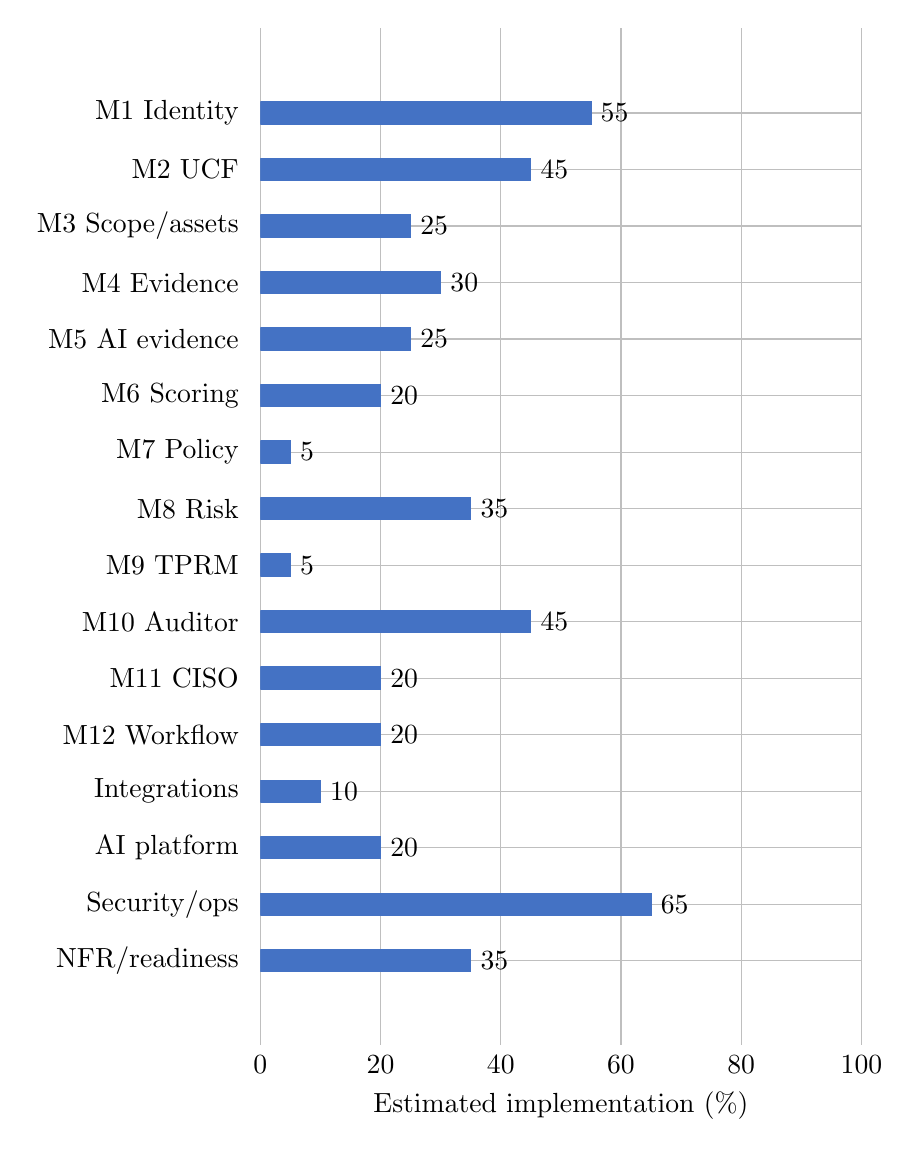
\begin{tikzpicture}
\begin{axis}[
  xbar,
  xmin=0,xmax=100,
  width=0.76\textwidth,
  height=14.5cm,
  bar width=8pt,
  xlabel={Estimated implementation (\%)},
  symbolic y coords={M1 Identity,M2 UCF,M3 Scope/assets,M4 Evidence,M5 AI evidence,M6 Scoring,M7 Policy,M8 Risk,M9 TPRM,M10 Auditor,M11 CISO,M12 Workflow,Integrations,AI platform,Security/ops,NFR/readiness},
  ytick=data,
  y dir=reverse,
  nodes near coords,
  nodes near coords align={horizontal},
  grid=major,
  axis line style={draw=none},
  tick style={draw=none},
]
\addplot[fill=blue,draw=blue] coordinates {
 (55,M1 Identity) (45,M2 UCF) (25,M3 Scope/assets) (30,M4 Evidence)
 (25,M5 AI evidence) (20,M6 Scoring) (5,M7 Policy) (35,M8 Risk)
 (5,M9 TPRM) (45,M10 Auditor) (20,M11 CISO) (20,M12 Workflow)
 (10,Integrations) (20,AI platform) (65,Security/ops) (35,NFR/readiness)
};
\end{axis}
\end{tikzpicture}
\end{center}

\small
\begin{longtable}{@{}>{\raggedright\arraybackslash}p{0.15\textwidth} >{\raggedright\arraybackslash}p{0.33\textwidth} >{\raggedright\arraybackslash}p{0.37\textwidth} >{\raggedleft\arraybackslash}p{0.05\textwidth}@{}}
\toprule
Workstream & Repository evidence & Principal remaining work & \% \\
\midrule
\endhead
M1 Tenancy \& identity & Tenant, organization, workspace, membership, invitations, tenant relationships, subscriptions, entitlements, engagements and scoped access. OIDC MFA claim enforcement and deny/log tests. & Full authentication lifecycle, SAML/SCIM, session policy, password recovery, IdP administration, vendor magic links, and complete persona UI. & 55 \\
M2 Unified Control Framework & Versioned framework/requirement/UCO/mapping models, evidence requirements, organisation controls, assignments, importer, fail-closed mapping tests. & Curated ISO 27001, PCI DSS, SOC 2 and DPDP content packs; structured delta analysis; mapping review workflow; domain-expert validation. & 45 \\
M3 Scope \& asset register & Application and engagement-scope records provide a narrow starting point. & Entities, locations, systems, processes, asset ownership, applicability rules, imports, lifecycle and dependency views. & 25 \\
M4 Evidence management & Immutable evidence/audit concepts, S3 storage, hashes, versioned Deployment Assurance artifacts and archive support. & General upload UX/API, AV/sandboxing, MIME/macro checks, OCR, classification, attributes, quality scoring, evidence timeline, remapping and large-file validation. & 30 \\
M5 AI evidence intelligence & AI run/model/prompt records, gateway boundaries and deterministic Deployment Assurance evaluation. & Candidate retrieval, vector/RAG pipeline, freshness/scope/sufficiency assessment, human quality gate, actionable requests, reuse analytics and evaluation corpus. & 25 \\
M6 Scores \& snapshots & Compliance summary and risk scores exist in limited paths. & Configurable compliance/maturity/evidence-quality models, daily snapshots, drill-down, comparisons, trends and what-if calculation. & 20 \\
M7 Policy lifecycle & Approval is a reusable primitive, but no material policy product was found. & Policy authoring, templates, AI review/drafting, approval workflow, publication, attestation, expiry and exception handling. & 5 \\
M8 Risk management & Risk, links, scores, remediation, tasks, acceptance and approval models; deterministic gap-to-risk/task behavior. & Full inherent/residual methodology, configurable matrices, treatment plans, heatmaps, imports, aggregation, KRIs and risk portal UX. & 35 \\
M9 TPRM & Vendor-campaign entitlement name only; no substantial vendor domain implementation found. & Vendor register/tiering, questionnaires, external portal, campaigns, response credibility, scoring, findings, continuous monitoring and reporting. & 5 \\
M10 Auditor workbench & Engagements, scope, members, status history, assignments, observations, verdicts, lock/unlock and cross-tenant audit events. & Full auditor/reviewer workbenches, allocation, AI briefs, sampling, findings/CAPA workflow, QA, engagement reporting and complete status UX. & 45 \\
M11 CISO cockpit & Basic compliance/risk presentation in the pilot client. & Governance/risk/compliance dashboards, framework comparison, maturity views, forecast/trend, board packs, alerting and configurable executive metrics. & 20 \\
M12 Workflow \& reports & Task and report records and basic APIs. & Recurrence, dependencies, escalation, notifications, report catalogue, rendering, scheduling, distribution and operational administration. & 20 \\
Integrations & API-first architecture and cloud-native deployment foundations. & Production connectors for identity, cloud, DevOps, ITSM, HRMS, security, SIEM, backup, LMS, communications and signature; common connector lifecycle. & 10 \\
AI platform & Isolated analyzer jobs, gateway/config/prompt/run records and deterministic-first assurance rules. & Governed model routing, schema enforcement across use cases, vector namespaces, prompt/evaluation operations, cost controls, red-team tests and golden datasets. & 20 \\
Security \& operations & RLS and cross-tenant tests; private EKS/CodeBuild design; Pod Identity; KMS storage; immutable cross-account checkpoints; replication/recovery IaC. & Merge and apply the stacked hardening changes, revoke old credentials, prove private deployment, perform cross-account negative tests, security testing, monitoring validation and timed recovery drill. & 65 \\
NFR/readiness & Container/Kubernetes paths, health checks, CI builds and a modular monolith suitable for pilot scale. & Availability SLO proof, scale/load tests, 250 MB evidence tests, WCAG AA, i18n, browser support, support operations, privacy/residency validation and certification evidence. & 35 \\
\bottomrule
\end{longtable}
\normalsize

\section{MVP cut-line status}

The concept note defines the core MVP differentiators as UCF mappings, evidence
extraction/versioning, evidence reuse, control assignment, and auditor verdict with
locking. Their estimated mean completion is 45\%.

\begin{center}
\begin{tabularx}{\textwidth}{X r X}
\toprule
MVP capability & Estimate & Assessment \\
\midrule
UCF and mappings & 45\% & Schema/import foundation exists; validated content and review lifecycle do not. \\
Evidence extraction and versioning & 30\% & Hash/version foundations exist; general OCR/classification pipeline does not. \\
Evidence reuse engine & 25\% & Control/evidence links exist; candidate retrieval and reuse intelligence remain. \\
Control assignment and scoped visibility & 70\% & Strongest MVP path, with explicit assignments and denial tests. \\
Auditor verdict and lock/unlock & 55\% & Core state and access behavior exist; full workbench, QA and reports remain. \\
\midrule
\textbf{Estimated MVP cut-line mean} & \textbf{45\%} & \\
\bottomrule
\end{tabularx}
\end{center}

\section{What is already working}

\begin{itemize}
  \item A modular Django/DRF backend with PostgreSQL RLS, composite tenant
  boundaries, cross-tenant denial tests, Redis/Celery, S3-compatible storage, and
  immutable audit events.
  \item SaaS tenant types, subscriptions and server-side entitlements; auditor
  engagements and member/scope enforcement; controlled verdict locking and
  reasoned manager unlock.
  \item UCF-related records, gap/risk/task linkage, evidence and assessment records,
  AI run governance records, and generic APIs over the implemented domain.
  \item Deployment Assurance normalizers, a twenty-rule baseline, deterministic
  evaluation/gates, OSCAL output, evidence hashes, waivers, decisions and drift
  concepts.
  \item A basic React pilot covering selected tenant, application, compliance,
  assurance, waiver and risk journeys.
  \item Local/container/Kubernetes/OpenShift/AWS deployment assets. The newest
  infrastructure branches add private EKS deployment, Pod Identity, immutable
  audit checkpoints and cross-region pilot-light recovery.
\end{itemize}

Repository verification at assessment time included 139 collected Python tests.
The latest recovery branch had a green full CI run, including frontend tests/build,
container builds, Kustomize rendering and Terraform tests. A disposable PostgreSQL
run had also exercised RLS. This is meaningful engineering evidence, but it does
not replace requirements acceptance or live-environment validation.

\section{What remains, in delivery order}

\subsection{1. Close the secure pilot path}

Merge the existing prerequisite and three hardening pull requests in order. Apply
them in staging, prove CodeBuild access after the EKS public endpoint is disabled,
verify that only the API/worker/checkpoint service accounts receive AWS identity,
revoke static S3 credentials, run cross-account read/overwrite/delete denial tests,
and complete a timed recovery drill. The current 1-hour RPO and 4-hour RTO are
targets until that drill succeeds; the concept note's stricter 15-minute RPO still
requires a product decision and measured proof.

\subsection{2. Turn the pilot into the stated MVP}

Create a signed-off SRS and requirement traceability matrix; supply expert-reviewed
framework packs; finish the general evidence ingestion/OCR/classification pipeline;
implement retrieval, reuse and human evidence review; finish scoring snapshots and
auditor workflows; and replace the single pilot screen with role-specific,
accessible journeys. Every business rule in the concept note should gain an
acceptance test.

\subsection{3. Add the broader GRC and TPRM product}

Build the asset/scope register, policy lifecycle, vendor/TPRM domain, mature risk
experience, workflow/notifications/reporting, CISO dashboards, board packs and the
highest-value connectors. Prioritize connectors from confirmed customers rather
than implementing the entire catalogue speculatively.

\subsection{4. Prove production readiness}

Run threat modelling, penetration and tenant-isolation tests; establish golden AI
datasets and quality thresholds; load-test stated scale and file sizes; prove SLOs,
backup/restore and regional recovery; complete accessibility and privacy/residency
reviews; and produce operational support and incident procedures.

\section{Indicative timeline}

The forecast assumes a stable 10--14 person cross-functional team, prompt product
decisions, access to the required AWS/security accounts, and domain experts able to
approve control content. Workstreams overlap; the chart shows elapsed weeks from an
assumed kickoff on 17 August 2026.

\begin{center}
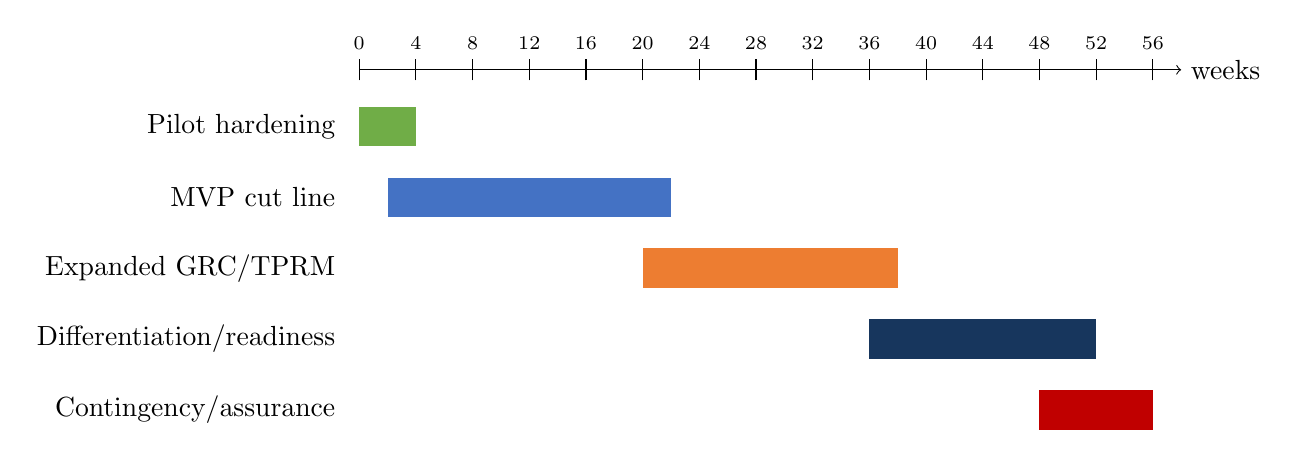
\begin{tikzpicture}[x=0.18cm,y=0.9cm]
  \draw[->] (0,0.8) -- (58,0.8) node[right]{weeks};
  \foreach \x in {0,4,...,56} {
    \draw (\x,0.65) -- (\x,0.95);
    \node[above,font=\scriptsize] at (\x,0.95) {\x};
  }
  \node[anchor=east] at (-1,0) {Pilot hardening};
  \fill[green] (0,-0.28) rectangle (4,0.28);
  \node[anchor=east] at (-1,-1) {MVP cut line};
  \fill[blue] (2,-1.28) rectangle (22,-0.72);
  \node[anchor=east] at (-1,-2) {Expanded GRC/TPRM};
  \fill[amber] (20,-2.28) rectangle (38,-1.72);
  \node[anchor=east] at (-1,-3) {Differentiation/readiness};
  \fill[navy] (36,-3.28) rectangle (52,-2.72);
  \node[anchor=east] at (-1,-4) {Contingency/assurance};
  \fill[red] (48,-4.28) rectangle (56,-3.72);
\end{tikzpicture}
\end{center}

\begin{center}
\begin{tabularx}{\textwidth}{p{0.20\textwidth}p{0.18\textwidth}X}
\toprule
Milestone & Target & Exit evidence \\
\midrule
Secure pilot closure & Sep 2026 & Staged private deployment, credential revocation, immutable checkpoint negative tests and first timed recovery evidence. \\
MVP cut line & Jan--Feb 2027 & Accepted UCF content, general evidence pipeline/reuse, scoring snapshots, assignments, auditor verdict/lock, core role journeys and traceable tests. \\
Expanded GRC/TPRM & May--Jun 2027 & Asset/scope, policy, vendor campaigns, risk, workflow/reporting, dashboards and priority connectors usable end to end. \\
Wider concept-note scope & Sep--Oct 2027 & AI quality proof, scale/SLO/DR evidence, accessibility/privacy work and production operating model. \\
\bottomrule
\end{tabularx}
\end{center}

\textbf{Confidence and alternatives.} Dates should be managed as ranges, not
commitments, until discovery and SRS sign-off. If the team is 4--6 people, expect
roughly 18--24 months. Delays in framework content, design, AI evaluation data,
security accounts, identity providers or vendor integrations sit on the critical
path.

\section{Prioritized next actions}

\begin{enumerate}
  \item Obtain review and merge the prerequisite PR, then merge the three stacked
  hardening PRs in order; repeat CI where historical runs were unavailable.
  \item Execute the staging and recovery runbooks and retain evidence. Reconcile
  the hardening plan's 1-hour RPO with the concept note's 15-minute NFR.
  \item Convert the concept note into a signed SRS and traceability matrix. Mark
  must/should/later and assign an acceptance test to every business rule.
  \item Run a two-week product/architecture inception for evidence, UCF, scoring,
  auditor and UX flows; lock the MVP cut line and measurable AI quality gates.
  \item Start framework content and golden-dataset work immediately because domain
  review, not coding, is likely to be the longest lead-time item.
  \item Deliver vertical slices: evidence upload to auditor verdict first; then
  policy/risk; then vendor campaign; then dashboards/reports and confirmed
  integrations.
\end{enumerate}

\section{Risks and decisions needed}

\begin{tabularx}{\textwidth}{p{0.17\textwidth}X X}
\toprule
Priority & Risk or decision & Required response \\
\midrule
Critical & The concept note is pre-SRS and leaves workflow, UX and acceptance details open. & Product, compliance and engineering sign-off on traceable requirements before committing dates. \\
Critical & Framework mappings and AI evidence judgments require expert-reviewed content and datasets. & Name content owners, license sources, establish golden datasets and record approval/version provenance. \\
Critical & Recovery and private-cluster changes are defined but not proven in the target accounts. & Merge/apply in order and run the staged access, negative-permission and timed DR tests. \\
High & Generic CRUD models can appear more complete than the user journey actually is. & Accept only end-to-end vertical slices with role, tenant, audit, failure and accessibility tests. \\
High & The full connector catalogue can consume the roadmap without validating demand. & Implement only contracted/high-frequency integrations first, behind one boring connector contract when a second connector proves the common shape. \\
High & The stated scale and 99.9\% availability have no production benchmark evidence. & Define workload models and run repeatable load, soak, failover and recovery tests before production claims. \\
Medium & Enterprise physical tenant isolation is deferred. & Keep shared RLS isolation for the pilot; add per-tenant database/bucket/KMS routing only for a contractual requirement. \\
\bottomrule
\end{tabularx}

\section{Evidence and limitations}

Evidence reviewed includes backend models, permissions, APIs and tests; Deployment
Assurance rules and tests; the React application; Docker, Kustomize and Terraform
assets; architecture/runbook documentation; and the current stacked infrastructure
branches. Relevant pull requests at assessment time were PRs \#28--\#31. PR \#31
had a green full CI result; PRs \#28--\#30 remained prerequisites or required
review/rerun. No claim in this report means those changes have been applied to a
live AWS environment.

This is a repository implementation assessment, not a compliance audit, penetration
test, legal opinion, formal capacity test, or certification readiness attestation.
Percentages should be replaced by accepted requirement counts once the SRS and
traceability matrix exist. Timeline estimates exclude procurement, certification,
customer onboarding, data migration, and delays outside the delivery team's control.

\vfill
\begin{center}
\small Source baseline: \textit{GRC/TPRM Platform Concept Note}, version 1.0,
53 pages, assessed against the \repo{} repository on 7 August 2026.
\end{center}

\end{document}
